% !Mode:: "TeX:UTF-8"%確保文檔utf-8編碼
%新加入的命令如下: reduline showendnotes 
%新加入的环境如下:solution solutionorbox solutionorlines solutionordottedlines

\documentclass[12pt]{exam}
\newlength{\textpt}
\setlength{\textpt}{12pt}

\usepackage{teachingplan}
\usetikzlibrary{positioning}

%输出方案 
%学生版 学霸版 老师版

%写上答案或者不写上答案%1  
\printanswers  

%提高题
%\includecomment{advanceexercises}
\excludecomment{advanceexercises}


\CenterWallPaper{1}{教案模板-2.pdf}

\newcommand{\keti}{功和机械能}
\newcommand{\zhongdian}{1.功 2.机械效率 3.功率  \\4.动能和势能 5.机械能及其转化}


\begin{document}
\ThisCenterWallPaper{1}{教案模板-1.pdf}
\vspace*{80pt}
\keti \par
\zhongdian \par
\section{杠杆和滑轮组分析}
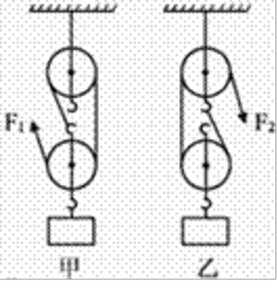
\includegraphics[scale=1]{图2} 

\begin{questions}
\setcounter{question}{3}
\question
(2012 福州)\\
小明用同一滑轮组分别将甲、乙两组钩码提升相同的高度,如下图所示。他两次提升钩码所用的拉力分别为F甲和F乙,则F甲\answerline*[<] F乙;所做的有用功分别为W甲和W乙,机械效率分别为η甲和η乙,则W甲\answerline*[<] W乙,η甲\answerline*[<] η乙。(均选填“>”、“=”或“<”)

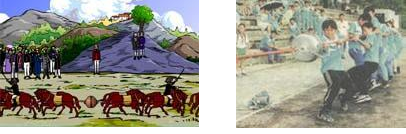
\includegraphics[scale=1]{图3} 

\question
(2012 常州)\\
分别用如下图所示的甲、乙两个滑轮组,在100s内将重为400N 的物体G匀速提升10m,每个滑轮的重均为20N。不计绳重及摩擦,此过程中(\answerline*[D])
\begin{multicols}{2}
\begin{figure}[H]
\centering
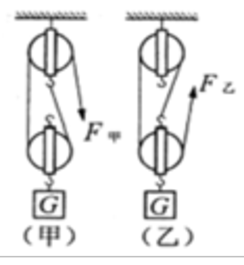
\includegraphics[width=0.6\linewidth]{图4}
\end{figure}
\columnbreak
\begin{choices}
\choice F甲做的功大于F乙做的功
\choice F甲做的功小于F乙做的功
\choice F甲做功的功率小于F乙做功的功率
\choice F甲做功的功率等于F乙做功的功率
\end{choices}

\end{multicols}
\end{questions}





\section{练习题}
\begin{questions}
\question
在下列情况中,物体既具有动能又具有重力势能的是(\answerline*[B])
\begin{choices}
\choice 海上航行的轮船
\choice 空中飞行的子弹
\choice 吊在天花板上的电灯
\choice 拉开的弓
\end{choices}

\question
下列各种情况中,属于动能转化为势能的是(\answerline*[D])
\begin{choices}
\choice “无边落叶萧萧下,不尽长江滚滚来”
\choice 空中匀速下降的跳伞运动员
\choice 拧紧的钟表发条带动指针走动
\choice 正在上升的滚摆
\end{choices}

\question
直升机在匀速下降过程中,能量变化情况是(\answerline*[B])
\begin{choices}
\choice 势能减少,动能增加,机械能不变
\choice 势能减少,动能不变,机械能减少
\choice 势能不变,动能不变,机械能不变
\choice 势能减少,动能不变,机械能不变
\end{choices}

\question
关于机械效率的说法正确的是(\answerline*[D])
\begin{choices}
\choice 越省力的机械,其机械效率越高
\choice 做的总功越多,机械效率越高
\choice 做的有用功越多,机械效率越高
\choice 有用功一定时,额外功越少,机械效率越高
\end{choices}

\question
奥运举重冠军陈小敏在比赛时,第一阶段她把100kg的杠铃很快地举过头顶,第二阶段使杠铃在空中稳稳地停留了3s,三名裁判都亮出了白灯,举重成功。关于她举重时对杠铃做功的情况,下列说法正确的是(\answerline*[B])
\begin{choices}
\choice 她在第一阶段内没有做功
\choice 她在第二阶段内没有做功
\choice 她在两个阶段内都做了功
\choice 她在两个阶段内都没有做功
\end{choices}

\question
下列单位中不是功的单位的是(\answerline*[C])
\begin{choices}
\choice W•s
\choice J
\choice J/s
\choice N•m
\end{choices}

\question
某人用手将一物体竖直举高2m和用机械效率为80%的斜面将它升高2m。比较两种情况(\answerline*[B])
\begin{choices}
\choice 用手举高时做功多
\choice 用斜面升高时做功多
\choice 两种情况做功一样多
\choice 两种情况都不做功
\end{choices}

\question
水电站修筑较高的拦河坝是为了\answerline*[增加水的势能]。

\question
上海桑塔纳牌小轿车的功率是:66 kW=\answerline*[66000]W=\answerline*[66000]J/s。\\“66kW”的物理意义是\answerline*[1秒钟做的功是66000J]。

\question
一辆小汽车与一辆装满货物的大卡车以相同的速度行驶,则小汽车的动能\answerline*[小于]大卡车的动能。(填“大于”“等于”或“小于”)

\question
跳水运动员从最高点向水面下落的过程中,他的\answerline*[势]能逐渐减少,\answerline*[动]能逐渐增加。

\question
弹簧门在推开后能自动关闭,这是由于门被推开后,弹簧被卷紧变形,具有\answerline*[弹性势]能;放手后,这个能转化为门的\answerline*[动]能,使门被关上。

\question
一只小鸟在空中飞行时具有40J的机械能,若它具有10J的势能,则它具有\answerline*[30]J的动能。

\question
小明在水平面上用50N的水平推力,加速推着一辆重120N的小车,前进了10m,小明的推力做功是\answerline*[500]J。水平面对小车的支持力做功是\answerline*[0]J。

\question
用一只铁桶从深井中取水,第一次取半桶,第二次取满桶,两次相比:W1额\answerline*[=]W2额,η1\answerline*[<]η2。(选填“>”“<”或“=”)

\question
在空气阻力不计的情况下,一只皮球从高处由静止下落,被地面弹起后不能再回到原来的高度。在整个过程中:
①说明皮球机械能的转化情况;
\begin{solutionorbox}[6ex]
皮球下落过程中:重力势能转化为动能,动能转化为弹性势能.皮球上升过程中:弹性势能转化为动能,动能转化为重力势能,机械能减少。
\end{solutionorbox}

②指出皮球在哪几个位置时的动能为零;
\begin{solutionorbox}[6ex]
在最高处时 动能全部转化为弹性势能处时反弹至最高处。
\end{solutionorbox}

③分析皮球不能回到原来高度的原因。
\begin{solutionorbox}[6ex]
皮球与地面碰撞过程中,一部分机械能转化为内能。
\end{solutionorbox}

\question
(2010 兰州)\\
如下图所示,物重G为 2000N,斜面长5m,高3m,斜面和滑轮组装置的总机械效率为80%,若将重物沿斜面以0.2m/s的速度拉上来,求:\\
(1)所需拉力 F 是多少? (2)机械的总功率是多少?
\begin{figure}[H]
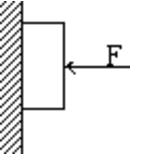
\includegraphics[width=0.3\linewidth]{图1}
\end{figure}
\begin{solution}[30ex]
如图知,动滑轮一端绳子的根数n=3.使用滑轮组时,自由端做的功是总功,直接提升物体做的功为有用功.不计摩擦和绳重时,克服动滑轮做的功为额外功.
  推算过程如下:
  (1)机械效率:
    ∵不计摩擦及绳重,∴F=(G物+G动)
    ∴G动=3F-G物=3×60-150=30N
  (2)绳端移动速度为:
     绳上的拉力F′=(G′物+G动)=(300+30)=110N
     ∴拉力的功率为P=F′·v=110×0.6=66W
答案:(1)83.3\%   (2)P=66W
\end{solution}


\question
(海南省)\\
跳绳是一项很好的体育健身活动,经测试重500N的某同学1min跳绳120次,每次离地约0.06m(每次离地高度和时间都相同)。\\
(1)该同学跳一次做功多少焦耳?\\
(2)他在这1 min的锻炼中消耗的功率是多大?\\
(3)跳绳时对地面的压强与站立时相比较有何变化?并说明判断的理由。
\begin{solution}[30ex]

\end{solution}

\end{questions}













\begin{advanceexercises}
\section{提高题}

\end{advanceexercises}

\ThisCenterWallPaper{1}{教案模板-3.pdf}

\end{document}



